\textbf{Onderbouw je antwoorden altijd door beredenering en/of berekening.}

Een driefasen asynchrone motor is aangesloten op een spanning van 400V/50Hz.
De motor drijft een last aan waarvan het koppel recht evenredig is met het toerental.
Bij het nominale toerental bedraagt het lastkoppel 100 Nm.
Voor de combinatie motor en last is het nominale toerental 1440 rpm.
Voor de motor geldt verder dat het aanloopkoppel 0,7 maal het nominale koppel is
$(T_{aanloop} = 0,7 \times T_{nom})$ en dat het kipkoppel gelijk is aan $T_{kip} = 2 \times T_{nom}$.

\begin{enumerate}
    \item [a.] \textbf{Wat is het aantal poolparen van deze motor? Bepaal de slip van de motor bij nominaal bedrijf.}
    
        Poolparen:
        $ P = \frac{60 \times f}{n_{s}} = \frac{60 \times 50}{\approx1440} \approx 2 poolparen $

        Slip:
        $slip 
        = \frac{n_{s} - n_{r}}{n_{s}} 
        = \frac{\frac{Hz*60}{P} - n_{r}}{\frac{Hz*60}{P}}
        = \frac{1500 - 1440}{1500} \times 100 
        = 4\% slip$

    \item [b.] \textbf{Bereken het nominale asvermogen.}

    $P_{nominale} 
    = \frac{T_{nominale} \times 2\pi \times n_{nominale}}{60}= \frac{100 \times 2\pi \times 1440}{60} 
    = 15079,65 Watt \approx 15 kW$


    \item [c.] \textbf{Teken in één grafiek: De koppeltoerenkarakteristiek van de motor en de koppeltoerenkarakteristiek van de last. Geef duidelijk de kenmerkende waarden aan en laat zien hoe je aan die waarden komt.}

        \begin{figure}[h]
            \centering
            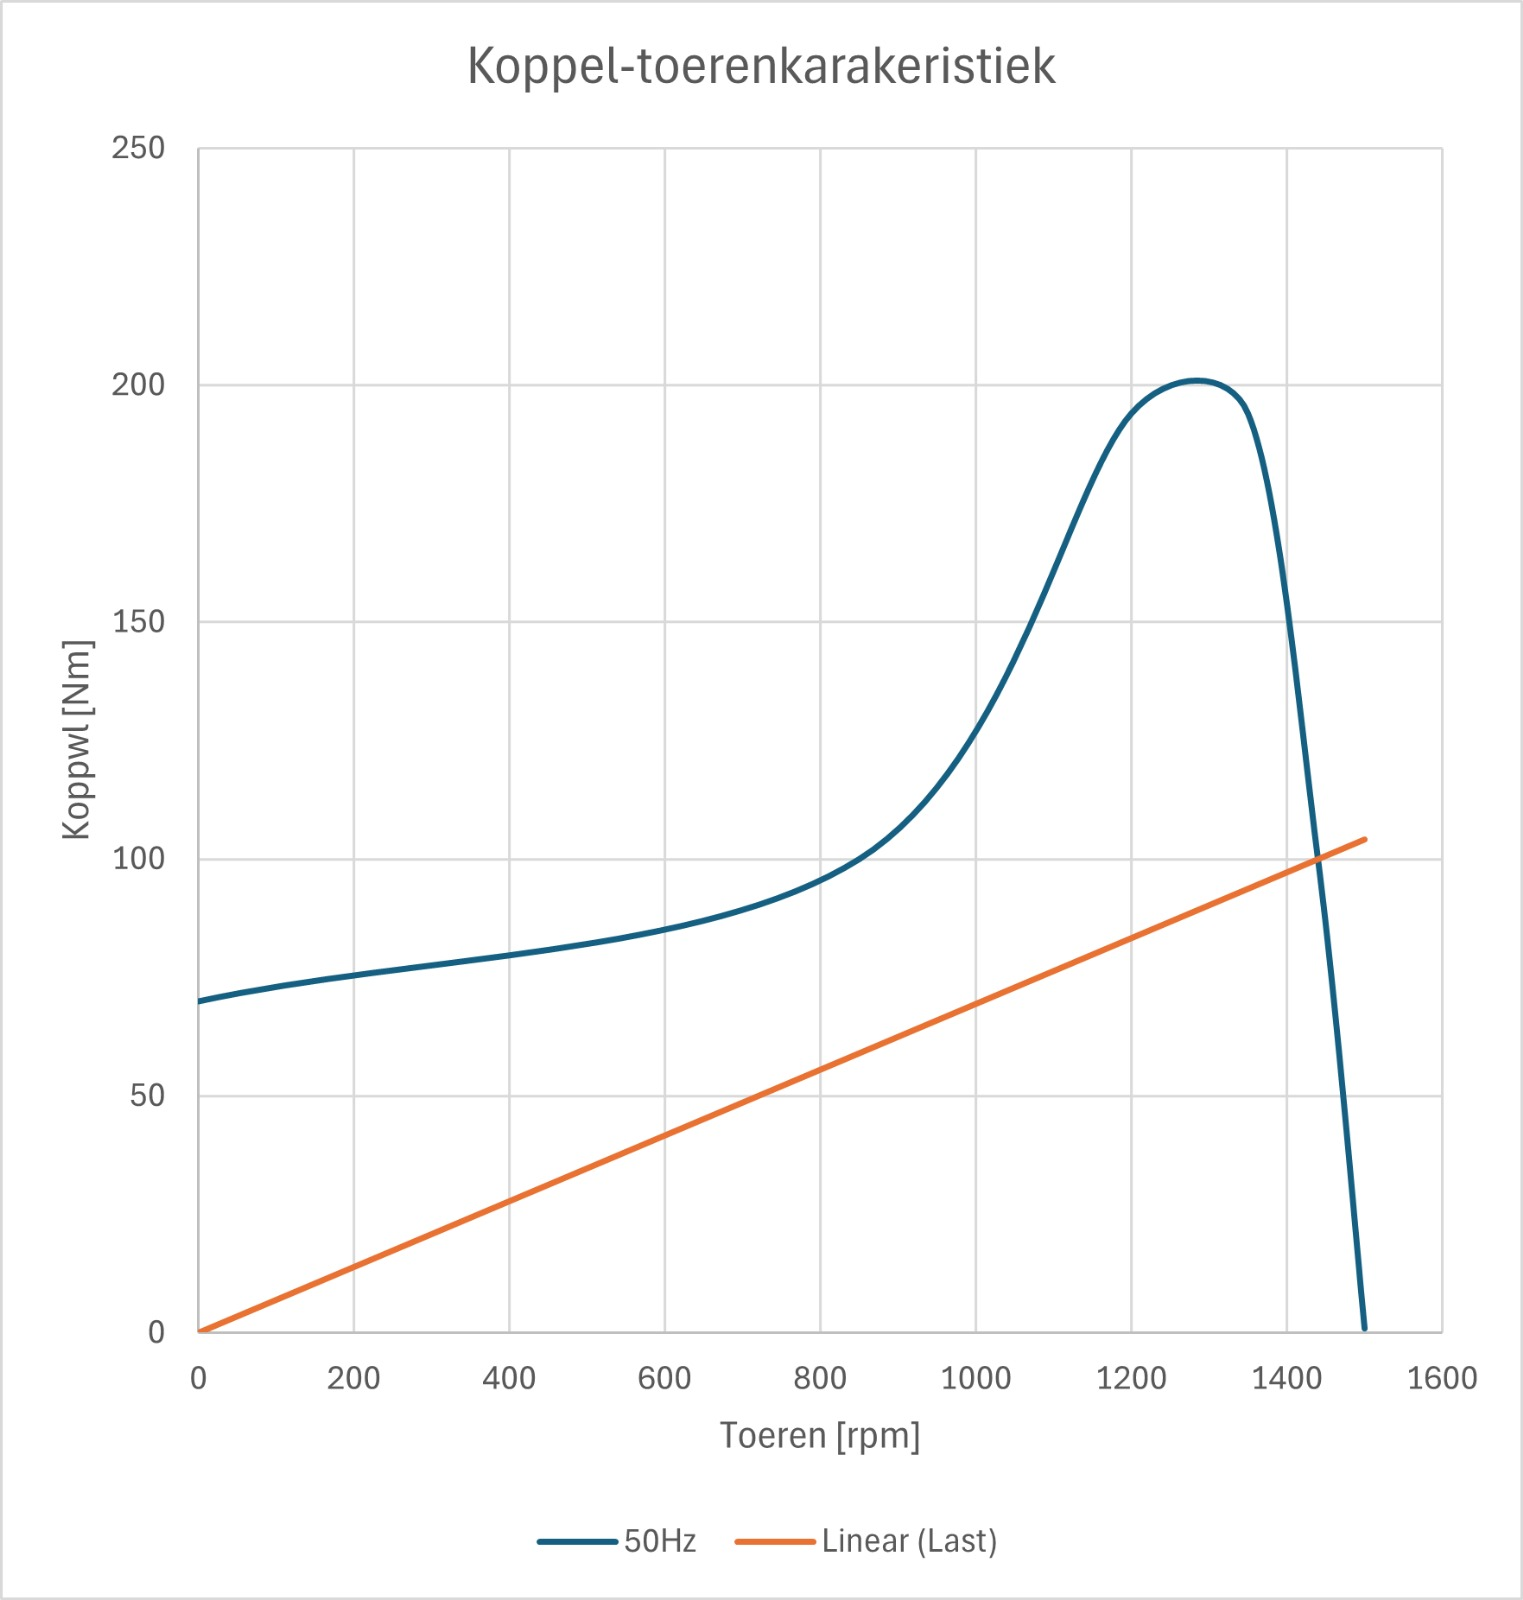
\includegraphics[scale=0.11]{kopppel-toerenkarakteristiek.jpg}
            \caption{koppel-toerenkarakteristiek}
        \end{figure}

    \item [d.] \textbf{Met behulp van een frequentieregelaar wordt het toerental gehalveerd $(n = 720 rpm)$. Wat moet de spanning en frequentie van de frequentieregelaar zijn om dit toerental in te kunnen stellen? Licht je antwoord kort toe.} 
        
        \[ frequentie 
        = \frac{n \times P}{60} 
        = \frac{720 \times 2}{60} 
        = 24 Hz \]
        
        Wat betreft de spanning, wordt deze meestal gehandhaafd op de nominale spanning van de motor, in dit geval \( 400 \, \text{V} \). De frequentieregelaar past de frequentie aan om het gewenste toerental te bereiken terwijl de spanning op het nominale niveau blijft om een goede werking van de motor te garanderen.
    

    \item [e.] \textbf{Wat verandert er aan de motorkarakteristiek als de frequentie van de frequentieregelaar $100 Hz$ is en de spanning gelijk blijft?
    Schets de nieuwe motorkarakteristiek en licht je antwoord kort toe.}

        \begin{figure}[h]
            \centering
            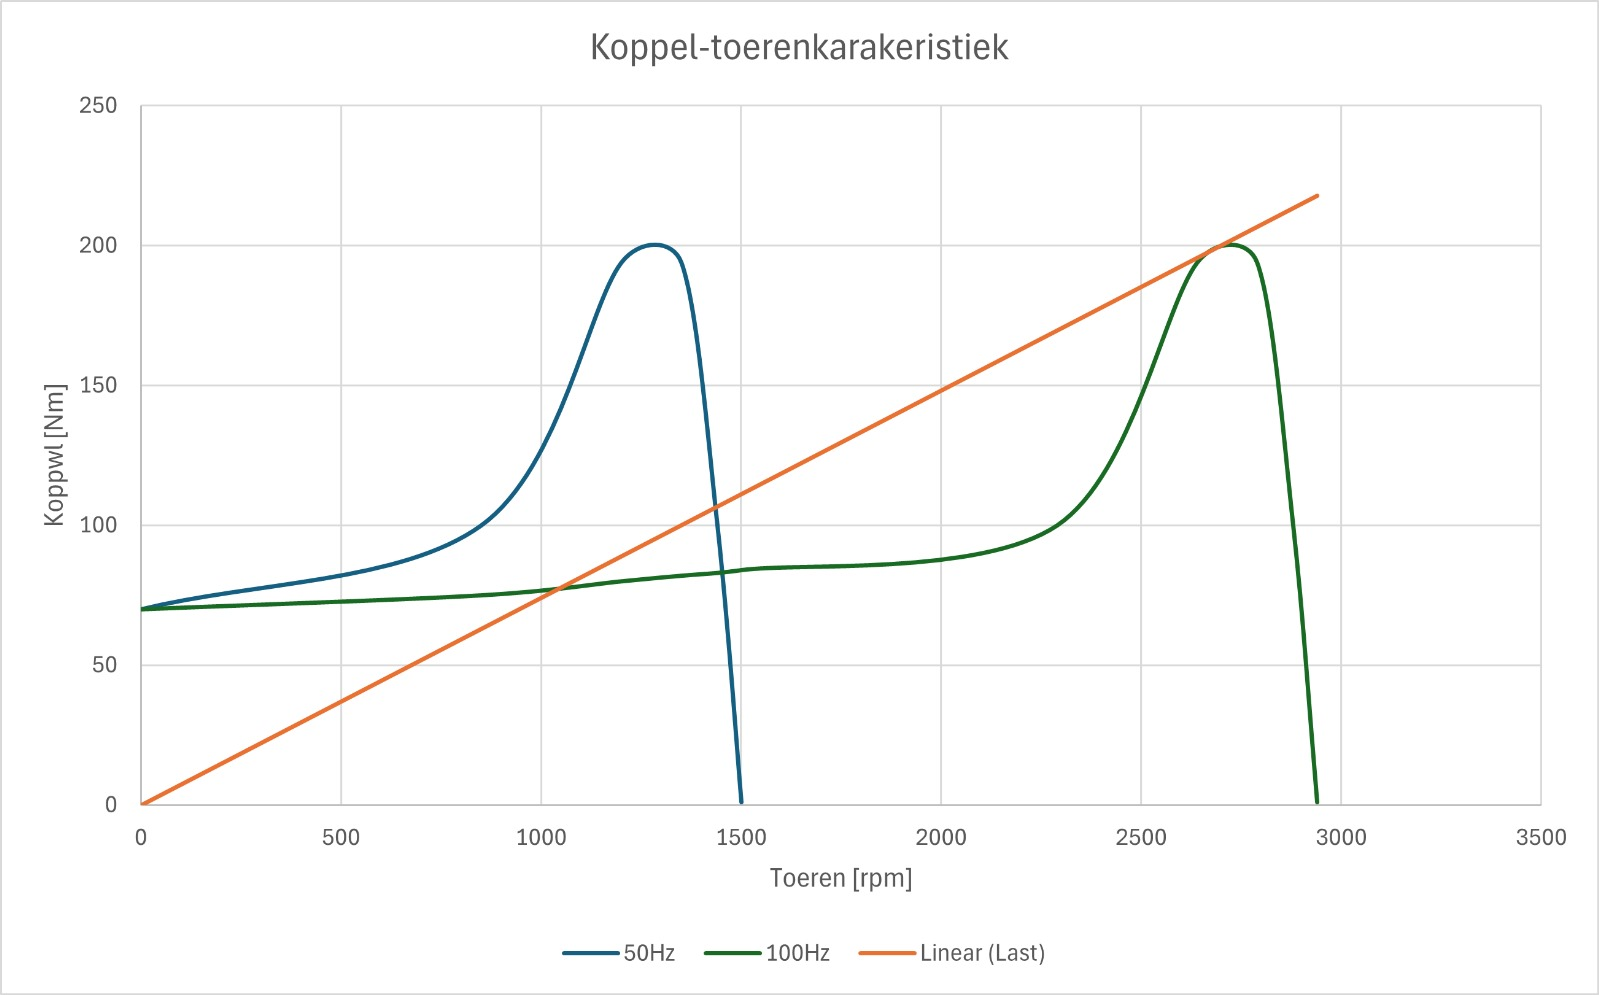
\includegraphics[scale=0.13]{2e.jpg}
            \caption{koppel-toerenkarakteristiek}
        \end{figure}

\end{enumerate}